\subsection{Customer Choice Dynamics}
We first show that every customer exhibits the following behavior: until (s)he reaches the phase transition point $i_0(t)$, she purchases from $A$ only due to the exogeneity paramater, and after that (s)he always purchases from $A$ till she receives the reward.
This behavior is cyclic, and repeats after every reward redemption.

\begin{lemma} $V(i)$ is an increasing function in $i$ if the following condition holds:
\begin{equation}
R > \frac{(1-\lambda)v}{1-\beta}
\end{equation}
And further, $V(i)$ can be evaluated as:
\begin{equation}
V(i) = \max\left\{ \frac{\lambda \beta V(i+1)+(1-\lambda)v}{1-(1-\lambda)\beta}, \beta V(i+1) \right\}
\end{equation}
\end{lemma}

\proof
First we show that $V(i)$ is an increasing function in $i$ by induction. We first show that if the condition above is satisfied, $V(k-1) < V(k) = R$. Suppose not, so $V(i) \geq R$. Then we have:
\begin{align*}
V(k-1) &= \lambda \beta V(k) + (1-\lambda)(v+\beta V(k-1)) \\
&= \frac{\lambda \beta R + (1-\lambda)v}{1-(1-\lambda)\beta} \\
&< \frac{\lambda \beta R + (1-\beta)R}{1-(1-\lambda)\beta} \\
&= \frac{R(1-(1-\lambda)\beta)}{1-(1-\lambda)\beta} = R
\end{align*}
But this is a contradiction, so $V(k-1) < V(k)$. Now assume $V(i+1) < V(i+2)$ for some $i < k-2$, we will show that this implies $V(i) < V(i+1)$. Suppose not, so $V(i) \geq V(i+1)$. As we did before we may upper bound $V(i)$.
\begin{align*}
V(i) &= \lambda \beta V(i+1) + (1-\lambda)(v+\beta V(i)) \\
&\leq (1-\lambda)v + \beta V(i) \\
\iff V(i) &\leq \frac{(1-\lambda)v}{1-\beta}
\end{align*}
But because $V(i+1) < V(i+2)$, we may lower bound $V(i+1)$.
\begin{align*}
V(i+1) &\geq \lambda \beta V(i+2) + (1-\lambda)(v+\beta V(i+1)) \\
&= (1-\lambda)v + (1-\lambda)\beta V(i+1) + \lambda \beta V(i+2) \\
&> (1-\lambda)+\beta V(i+1) \\
\iff V(i+1) &> \frac{(1-\lambda)v}{1-\beta}
\end{align*}
Again, we have a contradiction, so $V(i) < V(i+1)$, and $V(i)$ is an increasing function in $i$. Now we prove the second claim. We have the following:
\begin{align*}
V(i) &= \lambda \beta V(i+1) + (1-\lambda)\max\{v +\beta V(i), \beta V(i+1) \} \\
&= \max\{\lambda \beta V(i+1) + (1-\lambda)(v+\beta V(i)), \beta V(i+1) \}
\end{align*}

Assuming $V(i)$ is the left term in the above maximum, we may solve the equation for that term.
\begin{gather*}
V(i) = \lambda \beta V(i+1) + (1-\lambda)(v+\beta V(i)) \\
(1-(1-\lambda)\beta) V(i) = \lambda \beta V(i+1) + (1-\lambda)v \\
V(i) = \frac{\lambda \beta V(i+1) + (1-\lambda)v}{1-(1-\lambda)\beta}
\end{gather*}
And we get our claim.
\endproof

Now if the expected reward of the customer increases with the number of purchases made from $A$, we expect that at some number of purchases it becomes profitable for the customer to choose to purchase from $A$ as opposed to $B$.
We characterize this phase transition point in the following theorem.

\begin{theorem} Suppose $V(i)$ is an increasing function in $i$ and consider a customer with look-ahead parameter $t$. A phase transition occurs after (s)he makes $i_0(t)$ visits to firm $A$, where $i_0(t)$ is given by:
\begin{equation}
  i_0(t)=\begin{cases}
    k-\Delta \equiv i_0, & \text{if $t \geq \Delta$}.\\
    k-t, & \text{otherwise}.
  \end{cases}
\end{equation}
with 
\begin{align}
\Delta &= \left\lfloor \log_{\beta}\left(\frac{v}{R(1-\beta)}\right)\right\rfloor
\end{align}
\end{theorem}

\proof
First we solve for the condition on $V(i+1)$ for us to choose firm $A$ over $B$ willingly.
\begin{gather*}
\beta V(i+1) > \frac{\lambda \beta V(i+1) + (1-\lambda)v}{1-(1-\lambda)\beta} \\
\iff \beta V(i+1) \left(1-\frac{\lambda}{1-(1-\lambda)\beta} \right) > \left(\frac{1-\lambda}{1-(1-\lambda)\beta} \right) v \\
\iff \beta V(i+1) \left(\frac{1-(1-\lambda)\beta -\lambda}{1-(1-\lambda)\beta} \right) > \left(\frac{1-\lambda}{1-(1-\lambda)\beta} \right) v \\
\iff \beta V(i+1) \left(\frac{(1-\lambda)(1-\beta)}{1-(1-\lambda)\beta} \right) > \left(\frac{1-\lambda}{1-(1-\lambda)\beta} \right) v \\
\iff \beta V(i+1) > \frac{v}{1-\beta} \\
\iff V(i+1) > \frac{v}{\beta(1-\beta)}
\end{gather*}
Let $i_0$ be the minimum state $i$ such that the above holds, so in particular $V(i_0) \le \frac{v}{\beta(1-\beta)}$ but $V(i_0+1) > \frac{v}{\beta(1-\beta)}$. We know because $V$ is increasing in $i$, this point is indeed a phase transition: $V(i) > \frac{v}{\beta(1-\beta)}$ for all $i > i_0$, so after this point, the customer always chooses firm $A$. We may compute $V(i_0)$ easily using this fact.
\begin{equation*}
V(i_0) = \beta V(i_0+1) = \cdots = \beta^{k-i_0}V(k) = \beta^{k-i_0}R
\end{equation*}
Thus, we have the following:
\begin{gather*}
\beta^{k-i_0} \le \frac{v}{R\beta(1-\beta)} < \beta^{k-(i_0+1)} \\ 
\iff k-i_0 \ge \log_{\beta}\left(\frac{v}{R\beta(1-\beta)} \right) > k-(i_0+1) \\
\iff i_0 \le k - \log_{\beta}\left(\frac{v}{R(1-\beta)} \right) + 1 < i_0 + 1\\
\iff i_0 = k - \left\lfloor \log_{\beta}\left(\frac{v}{R(1-\beta)}\right) \right\rfloor \equiv k-\Delta
\end{gather*}

The above dependence reduces to the following after incorporating the look-ahead distribution:

\begin{equation*}
  i_0(t)=\begin{cases}
    i_0, & \text{wp } p,\\
    k, & \text{wp } 1-p.
  \end{cases}
\end{equation*}
\endproof

Note that the phase transition point is independent of $\lambda$, the customer's visit probability bias toward the merchant.
As we would expect, it increases with the look-ahead parameter, and with the price discount offered by merchant $B$.
Additionally, it decreases with an increase in the reward value $R$ and a decrease in the distance to reward $k$.
The variation with the discount factor $\beta$ is interesting: we can show that for any $\frac{R}{v} \ge 1$ there exists a $\beta \in [0,1]$ that minimizes the phase transition point $i_0$ for ''forward-looking'' customers.
This means that customers who are more patient have a longer time frame to transition and so do customers who are less patient than the optimal value.
We refer to the ratio of number of visits required for a forward-looking customer to adopt a reward program and the total distance to the reward as the ``influence zone''.
Intuitively this is the fraction of visits that the merchant wants to influence the customer by offering exogenous means of earning additional points like bonus miles in airlines, or accelerated earnings, as discussed in the introduction.
Next we find the optimal $k$ for minimizing this influence zone.

\begin{remark}\label{rem:inf_zone}
Influence zone is minimized at $k = \frac{e}{\alpha(1-\beta)}$ under proportional promotion budgeting. 
\end{remark}
\proof
As defined the influence zone is $\frac{i_0}{k} = \frac{k-\Delta}{k} = 1 -\frac{\Delta}{k}$.
Thus minimizing the influence zone is equivalent to maximizing $\frac{\Delta}{k}$.
\begin{align*}
\frac{\Delta}{k} = \frac{\log_\beta\left(\frac{1}{\alpha k(1-\beta)}\right)}{k}\sim \frac{\log (\alpha k(1-\beta))} {k(1-\beta)}
\end{align*}
The above approximation relies on $\beta$ close to 1. Now this value is maximized at $k = \frac{e}{\alpha(1-\beta)}$. Therefore, for all $b$, the optimal value for $k$ is given by $\frac{e}{\alpha(1-\beta)}$, the value for which $\frac{\Delta}{k}$ is maximized and takes the value $\frac{\alpha}{e}$. 
At this value the influence zone takes the value $1-\frac{\alpha}{e}$.
\endproof
Note that if $\alpha$ is $1$, then the value of $k$ corresponds to a cashback between $2$\% and $4$\% as $\beta$ ranges between $0.95$ and $0.9$.
This value is realistic to what is observed in practice.


\subsection{Merchant Objective Dynamics}

\subsubsection{Optimizing Reward Parameters}

So far we have characterized the customer behavior within the duopoly without concern about the particular reward design parameters. 
In this section, we derive optimal parameters for the reward program design with the objective of maximizing the revenue of the reward program merchant. 
Interestingly, we see that maximizing revenue corresponds to minimizing the influence zone, as illustrated above.

\begin{theorem}
Under proportional promotion budgeting, the optimal reward distance ($k$) and the optimal budget proportion ($\alpha$) for merchat $A$ follow the relation $\alpha k = \frac{e}{(1-\beta)}$ at all values of $b$ as long as $\beta$ is close to 1.
\end{theorem}
\proof
Let $\theta = \frac{\Delta}{k}$. First, we evaluate $RoR_A$.
We substitute the value of the phase transition point obtained above in the rate of revenue equation for $A$ to reevaluate it. 
And since we assume that $\lambda$ and $t$ are drawn independent of each other, we can separate the expectation terms and evaluate them sequentially, first over $t$, then over $\lambda$.
\begin{align*}
RoR_A =& \underset{\lambda, t}E\left[\frac{k-R}{i_0(t)/\lambda + k - i_0(t)}\right]\\
                                       =& \underset{\lambda}E\left[p\cdot\frac{k-R}{i_0/\lambda + k - i_0} + (1-p)\frac{\lambda(k-R)}{k}\right]\\
                                       =& \underset{\lambda}E\left[p\cdot\frac{\lambda(k-R)}{k\lambda + i_0(1-\lambda)} + (1-p)\frac{\lambda(k-R)}{k}\right]\\
                                       =& \underset{\lambda}E\left[p\cdot\frac{\lambda(1-\alpha v)}{1-\theta(1-\lambda)} + (1-p)\lambda (1-\alpha v)\right]\\
\end{align*}

Observe that the term inside the expectation is maximized when $\theta$ is maximized.
Using Leibniz' Rule, we can conclude that the integral itself is maximized when $\theta$ is maximized, which as shown above, is equivalent to minimizing the influence zone.
As shown in Remark~\ref{rem:inf_zone}, this happens at $k \alpha = \frac{e}{1-\beta}$. 
And at this point, $\theta = \frac{\Delta}{k} = \frac{\alpha}{e}$.
\endproof

An interesting point to observe above is that if $\alpha$ is constant, then maximizing the revenue objective is equivalent to minimizing the influence zone.
This result matches the following intuition - the faster the merchant can get customers to adopt the reward program, the more transactions it will make in the long run - but is stronger as it actually maximizes the revenue objective as well. 
Although, reward point accelerations are common and effective mechanisms to get customers to adopt reward programs, we have shown that designing the reward program so that a minimum number of such accelerations is required, leads to maximizing merchant's revenue. 
The condition that $\beta$ be close to 1 is not very restrictive, as the discount factor is expected to be high in most cases. 
Note that because $k \geq \Delta$, the above also shows $\alpha \leq e$. 
Finally, observe that we need $R > \frac{(1-\lambda)v}{1-\beta}$ for $V$ to be increasing. 
We meet this condition with proportional budgeting when $k = \frac{e}{\alpha(1-\beta)}$ as $R = \alpha k v = \frac{e v}{1-\beta} \geq \frac{v}{1-\beta} \geq \frac{(1-\lambda)v}{1-\beta}$. 

The above framework can be used for optimizing for the reward parameters to maximize $A$'s rate of revenue, for varying distributions of the customer population.
That is, if a merchant has a good estimate of its customer population's distribution, it can easily utilize the above theorem to optimize its reward scheme.
We leave the competitive study where merchant $B$ could strategize on its discount value $v$ for future work.

Figure~\ref{fig:alpha_max} shows how the rate of revenue of the reward merchant varies as a function of $\alpha$, after fixing $\alpha k$ as in our previous theorem, for various distributions of excess loyalty. For all three distributions we observe three general behaviors of $RoR_A$: for large values of $v$, the rate of revenue decreases along all feasible values of $\alpha$; for small values of $v$, the revenue increases for all values of $\alpha$; and for some values of $v$ in between, the revenue is convex with a minimizer in $(0, e)$. We believe that $RoR_A$ will always depend on $\alpha$ in one of these three ways. That is, no distribution will maximize the revenue at some $\alpha \in (0,e)$, so if $\alpha$ is not fixed, the reward merchant should always set $\alpha$ to $e$ or 0 -- corresponding to no reward program.
Note that the exact values of $v$ for which these behaviors occur depend also on $p$ and the parameters of the specific distribution. In the following subsection, we explore these conditions for the uniform distribution for fixed $\alpha$. 

\begin{figure*}[t!]
\centering
\begin{subfigure}[t]{0.5\textwidth}
\centering
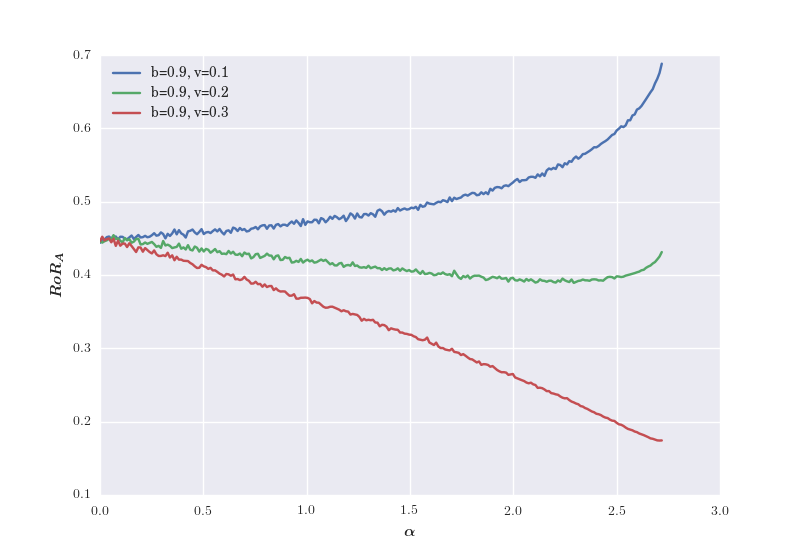
\includegraphics[height=2in]{./figures/rora_alpha_unif_v2.png}
\caption{Uniform distribution.}
\end{subfigure}%
~ 
\begin{subfigure}[t]{0.5\textwidth}
\centering
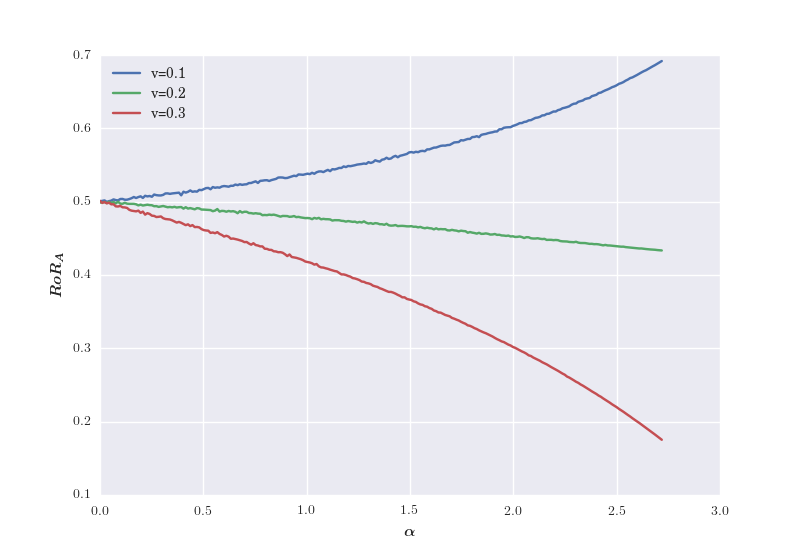
\includegraphics[height=2in]{./figures/rora_alpha_normal_v2.png}
\caption{Normal distribution.}
\end{subfigure}
\centering
\begin{subfigure}[t]{0.5\textwidth}
\centering
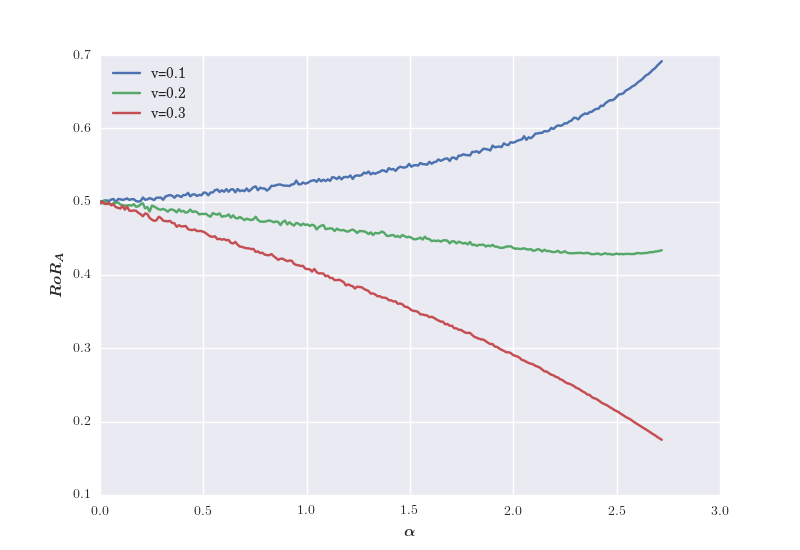
\includegraphics[height=2in]{./figures/rora_alpha_logit_v2.png}
\caption{Logit-normal distribution.}
\end{subfigure}

\caption{{Rate of revenue for reward merchant as a function of $\alpha$ (with $k = \frac{e}{\alpha(1-\beta)}$) for different distributions. For all distributions, $\beta = 0.9$, $p = 0.9$ and $v$ varies as labeled. The uniform distribution is on $(0,b]$ with $b = 0.9$; the normal distribution has $\mu = 0.5$ and $\sigma = 0.1$; and the logit-normal distribution is the standard on $[0,1]$.}}
\label{fig:alpha_max}
\end{figure*}

\subsubsection{Revenue Comparisons}

Now we characterize conditions for when it is strictly better for $A$ to offer a reward program for a specific distribution of the loyalty bias parameter - when $\lambda$ for every customer is drawn uniformly at random between $(0,b]$ where $b$ is less than $1$. We will assume this distribution for the remainder of the section.
This condition boils down to two situations: first, the rate of revenue for $A$ should be higher than that of $B$ and second, that the rate of revenue for $A$ should be higher than it could have achieved by not offering the reward program at the same fixed price.
First, we evaluate the expected rates of revenue for both $A$ and $B$ under the optimality relation between $k$ and $\alpha$ mentioned above with $\lambda$ being drawn from a uniform distribution.

\begin{align*}
RoR_A =& \underset{\lambda}E\left[p\cdot\frac{\lambda(1-\alpha v)}{1-\theta(1-\lambda)} + (1-p)\lambda (1-\alpha v)\right]\\
      =& pk\cdot\frac{1-\alpha v}{\Delta}\cdot\left(1 - \frac{k-\Delta}{b\Delta}\log\left(1+\frac{b\Delta}{k-\Delta}\right)\right) + (1-p)\frac{bk(1-\alpha v)}{2k}\\
      =& (1-\alpha v) \left(p\frac{e}{\alpha}\left(1-\frac{e-\alpha}{b\alpha}\log\left(1+\frac{b\alpha}{e-\alpha}\right)\right) + (1-p)\frac{b}{2}\right)
\end{align*}

\begin{align*}
RoR_B =& \underset{\lambda, t}E\left[\frac{(i_0(t)\lambda - i_0(t))(1-v)}{i_0(t)/\lambda + k - i_0(t)}\right]\\
      =& \underset{\lambda}E\left[p\cdot\frac{(i_0/\lambda - i_0)(1-v)}{i_0/\lambda + k - i_0} + (1-p)\frac{(k/\lambda - k)(1-v)}{k/\lambda}\right]\\
      =& \underset{\lambda}E\left[p\cdot\frac{i_0(1-\lambda)(1-v)}{k\lambda + i_0(1-\lambda)} + (1-p)(1-\lambda)(1-v)\right]\\
      =& p\cdot\frac{i_0(1-v)}{b(k-i_0)^2}\left(k\log\left(1+\frac{b(k-i_0)}{i_0}\right) - b(k-i_0)\right) + (1-p)(1-\frac{b}{2})(1-v)\\
      =& p\cdot\frac{(k-\Delta)(1-v)}{b\Delta^2}\left(k\log\left(1+\frac{b\Delta}{k-\Delta}\right) - b\Delta\right) + (1-p)(1-\frac{b}{2})(1-v)\\
      =& p\cdot\frac{(k-\Delta)(1-v)}{\Delta}\left(\frac{k}{b\Delta}\log\left(1+\frac{b\Delta}{k-\Delta}\right) - 1\right) + (1-p)(1-\frac{b}{2})(1-v)\\
      =& p\cdot\frac{(k-\Delta)(1-v)}{\Delta}\left(\frac{k}{b\Delta}\log\left(1+\frac{b\Delta}{k-\Delta}\right) - 1\right) + (1-p)(1-\frac{b}{2})(1-v)\\
      =& (1-v)\left(p\cdot\frac{e-\alpha}{\alpha}\left(\frac{e}{b\alpha}\log\left(1+\frac{b\alpha}{e-\alpha}\right) - 1\right) + (1-p)(1-\frac{b}{2})\right)\\
      =& (1-v)\left(p\frac{e}{\alpha}\left(\frac{e-\alpha}{b\alpha}\log\left(1+\frac{b\alpha}{e-\alpha}\right) - \frac{e-\alpha}{e}\right) + (1-p)(1-\frac{b}{2})\right)
\end{align*}

\begin{comment}
Under approximation get:

\begin{align*}
RoR_A \sim & \frac{b}{2}(1-\alpha v)\left(\frac{pe}{e-\alpha} + (1-p)\right)\\
      \sim & \frac{b}{2}(1-\alpha v) \left(1 + \frac{p\alpha}{e-\alpha}\right)\\
       \sim & \frac{b}{2}\left(1-\alpha v + \frac{p\alpha}{e-\alpha} - \frac{pv\alpha^2}{e-\alpha}\right)
\end{align*}

Maximizing above gives:

\begin{align*}
& -v + \frac{ep}{(e-\alpha)^2} - \frac{(e-\alpha)2pv\alpha + pv\alpha^2}{(e-\alpha)^2}\\
&= -v + \frac{ep}{(e-\alpha)^2} - \frac{pv\alpha(2e-\alpha)}{(e-\alpha)^2} = 0\\
&\implies ep - 2pe\alpha v + pv\alpha^2 = v(e^2 - 2e\alpha + \alpha^2)\\
&\implies e(p-ev) = (\alpha^2 v - 2e\alpha v)(1-p)\\
&\implies \alpha^2 - 2e\alpha = \frac{e(p-ev)}{v(1-p)}\\
&\implies (e-\alpha)^2 = \frac{ep - e^2v + e^2 v - e^2 vp}{v(1-p)}\\
&\implies (e-\alpha)^2 = \frac{ep(1-ev)}{v(1-p)}\\
&\implies \alpha = e - \sqrt{\frac{ep(1-ev)}{v(1-p)}}
\end{align*}
\end{comment}

Observe that both the above equations have a left term and a right term. The left term is the rate of revenue obtained from strategic customers whereas the right term is that obtained from the myopic customers.
As $\alpha$ ranges between $0$ and $e$, the value on the left term increases from $0$ for $RoR_A$ and decreases to $0$ for $RoR_B$.
That is, by controlling the reward budget ratio, $A$ is able to gain the entire strategic customer base.
But now observe how $RoR_A$ varies with $\alpha$:
the marginal revenue term $(1-\alpha v)$ decreases with $\alpha$ as the merchant gives higher rewards to customers, but the market share term increases as $A$ gains more strategic customer revenue by decreasing the tipping point time with an increase in the reward budget.
As $\alpha \to 0$, $RoR_A \to b/2$, \ie, the revenue earned is only due to visit probability bias, and is equivalent to the reveue earned by $A$ when not running any reward program.

Figure~\ref{fig:offer_reward_or_not} illustrates the region in terms of the customer parameters $(b,p)$ where it is better for $A$ to offer a reward program, \ie, $RoR_A > RoR_B$ (indicated in blue) and $RoR_A > \frac{b}{2}$ (indicated in yellow) for different values of $\alpha$, keeping $v = 0.05$ and $\beta = 0.95$ fixed.
The blue region shows that there is a clear threshold of $b$ and $p$ values beyond which $RoR_A > RoR_B$.
But more interestingly, the threshold value of $b$ and $p$ decreases as $\alpha$ is increased toward $e$.
Whereas the yellow region shows that if the fraction of strategic customers is not too small, the firm should choose to run a reward program most of the time except for when $b$ is large; larger $b$ values mean that customers make more exogenous visits, so a reward program is no longer needed to entice visits, but only decreases the profits of the reward program merchant.
The intersection of two regions, \ie, the region in green, indicates that the range of values of $b$ for which the reward program is strictly profitable increases as $p$ increases.
We formally show this result next.

\begin{figure*}[t!]
\centering
\begin{subfigure}[t]{0.5\textwidth}
\centering
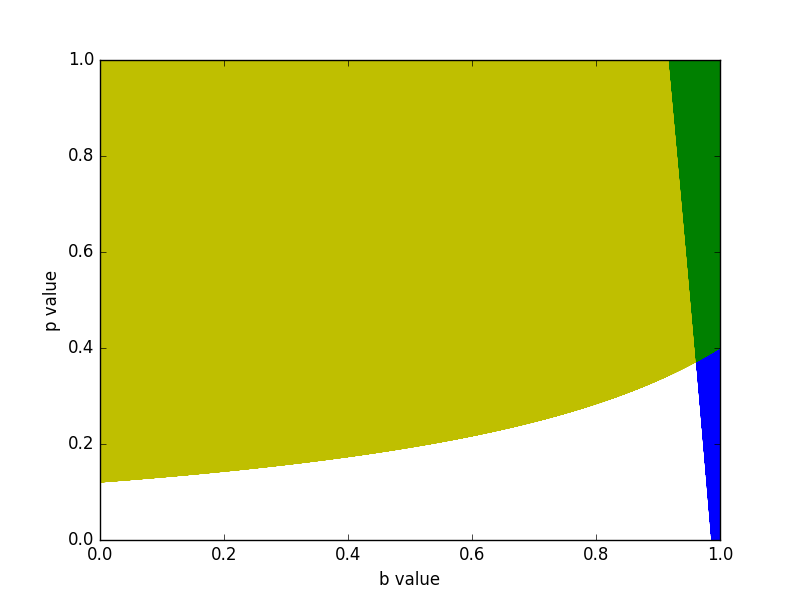
\includegraphics[height=2in]{./figures/bp_pair_both_al0p5.png}
\caption{$\alpha = 0.5$}
\end{subfigure}%
~ 
\begin{subfigure}[t]{0.5\textwidth}
\centering
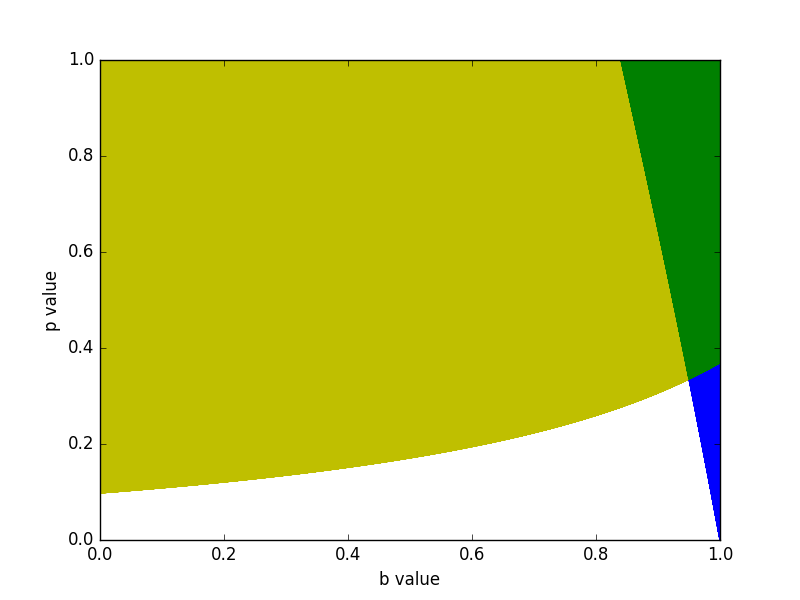
\includegraphics[height=2in]{./figures/bp_pair_both_al1p0.png}
\caption{$\alpha = 1$}
\end{subfigure}
\centering
\begin{subfigure}[t]{0.5\textwidth}
\centering
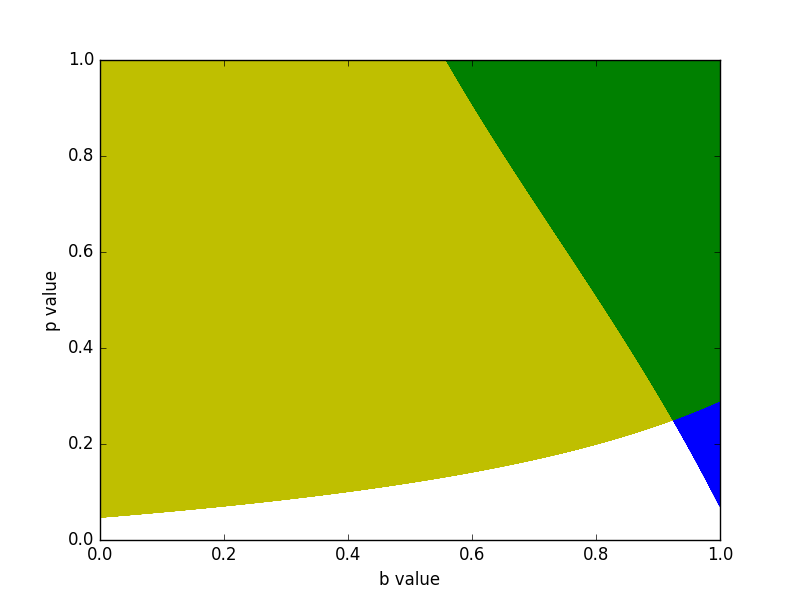
\includegraphics[height=2in]{./figures/bp_pair_both_al2p0.png}
\caption{$\alpha = 2$}
\end{subfigure}%
~ 
\begin{subfigure}[t]{0.5\textwidth}
\centering
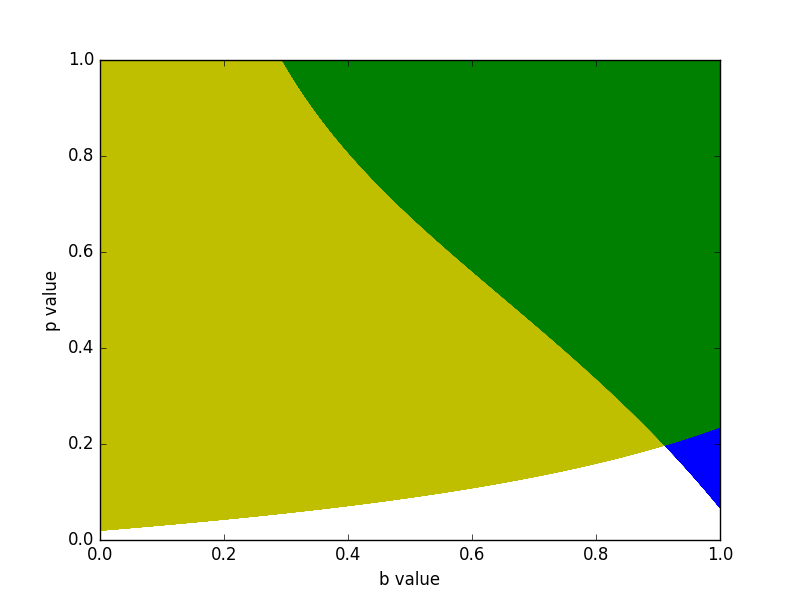
\includegraphics[height=2in]{./figures/bp_pair_both_al2p5.png}
\caption{$\alpha = 2.5$}
\end{subfigure}

\caption{{Regions where $RoR_A > RoR_B$ (blue), where $RoR_A > \frac{b}{2}$ (yellow) and where both are true (green) for different values of $\alpha$. In all cases, $\beta = 0.95$, $v = 0.05$ and $\lambda$ drawn uniformly on $(0,b]$.}}
\label{fig:offer_reward_or_not}
\end{figure*}

\begin{figure*}[t]
\centering
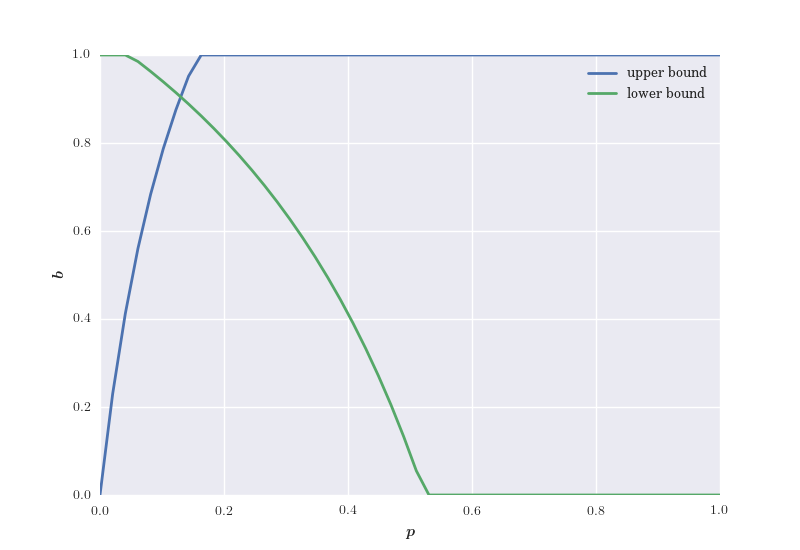
\includegraphics[scale = 0.4]{./figures/b_region_v2.png}
\caption{The upper and lower bounds on $b$ as a function of $p$. Here $v = 0.05$ and $\alpha \rightarrow e$.}
\label{fig:b_region}
\end{figure*}

For any fixed $\alpha$, the exact conditions on $p$, $b$ and $v$ for $RoR_A > RoR_B$ and $RoR_A > \frac{b}{2}$ are rather complex. We will first focus on one particular simple case: $\alpha \rightarrow e$. 

\begin{lemma}
As $\alpha \rightarrow e$, $RoR_A > RoR_B$ if and only if the following condition on $b$ holds:
\begin{equation}
b > 2\cdot \frac{(1-v) - \frac{p}{1-p}\cdot (1-ev)}{(1-v) + (1-ev)}
\end{equation}
\end{lemma} 
\proof
First we compute the following quantity.
\begin{equation*}
\lim_{\alpha \to e} \frac{e-\alpha}{b\alpha}\log\left(1+\frac{b\alpha}{e-\alpha}\right)
\end{equation*}
Let $\frac{e-\alpha}{b\alpha} = x$, then it is easy to see that the above limit is equivalent to $\lim_{x\to \infty} \frac{\log(1+x)}{x} = 0$. Then as $\alpha \rightarrow e$, we have the following expressions for $RoR_A$ and $RoR_B$.
\begin{equation*}
RoR_A = (1-ev)\left(p+(1-p)\frac{b}{2} \right)
\end{equation*}
\begin{equation*}
RoR_B = (1-v)(1-p)\left(1-\frac{b}{2} \right)
\end{equation*}
And our condition $RoR_A > RoR_B$ simplifies.
\begin{align*}
(1-ev)\left(p+(1-p)\frac{b}{2} \right) &> (1-v)(1-p)\left(1-\frac{b}{2} \right) \\
\frac{b}{2}(1-p)(1-ev+1-v) &> (1-v)(1-p)-(1-ev)p \\
b &> 2\cdot \frac{(1-v) - \frac{p}{1-p}\cdot (1-ev)}{(1-v) + (1-ev)} 
\end{align*}

\endproof

The above lemma gives a lower bound on $b$ for $RoR_A > RoR_B$ in terms of $p$ and $v$. In order for the reward program to be strictly better than the traditional pricing model, we also need $RoR_A > \frac{b}{2}$. The following lemma shows that this condition gives a corresponding upper bound on $b$.

\begin{lemma}
As $\alpha \rightarrow e$, $RoR_A > \frac{b}{2}$ if and only if the following condition on $b$ holds:
\begin{equation}
b < \frac{2p}{p+\frac{ev}{1-ev}}
\end{equation}
\end{lemma} 

\proof
The condition $RoR_A > \frac{b}{2}$ is equivalent to:
\begin{align*}
(1-\alpha v)\left(p \frac{e}{\alpha}\left(1-\frac{e-\alpha}{b\alpha}\log \left(1+\frac{b\alpha}{e-\alpha} \right) \right)+(1-p)\frac{b}{2}\right) &> \frac{b}{2} \\
\frac{e}{\alpha} \left(1-\frac{e-\alpha}{b\alpha}\log \left(1+\frac{b\alpha}{e-\alpha} \right) \right) &> \frac{b}{2p}\left(\frac{1}{1-\alpha v}-(1-p) \right)
\end{align*}
As $\alpha \rightarrow e$, the left term above approaches 1 and we are left with:
\begin{align*}
b &< \frac{2 p (1-ev)}{1-(1-p)(1-ev)} \\
&= \frac{2p(1-ev)}{p-pev+ev} \\
&= \frac{2p}{p+\frac{ev}{1-ev}}
\end{align*}
\endproof

The previous two lemmas provide lower and upper bounds on $b$ for $RoR_A > RoR_B$ and $RoR_A > \frac{b}{2}$, respectively. For the reward program to be strictly better than all alternatives, both of these conditions must be met. We combine them to get an intuitive necessary and sufficient condition on $p$ for the reward program to be ``strictly better''. 

\begin{lemma}
As $\alpha \rightarrow e$, for the reward program to be strictly better on some values of $b$, a necessary and sufficient condition on $p$ is:
\beq
\label{eq:necp}
p > 1 - \frac{1-ev}{1-ev^2}
\eeq
\end{lemma}

\proof
 The values of $b$ for which both previous lemmas are met is given by:
\begin{align*}
2\cdot \frac{(1-v) - \frac{p}{1-p}\cdot (1-ev)}{(1-v) + (1-ev)} < b < \frac{2p}{p+\frac{ev}{1-ev}}
\end{align*}
The above inequality is only valid when the lower bound is less than the upper bound. We may manipulate this inequality to get the simple condition on $p$ in our claim.
\begin{align*}
2\cdot \frac{(1-v) - \frac{p}{1-p}\cdot (1-ev)}{(1-v) + (1-ev)} &< \frac{2p}{p+\frac{ev}{1-ev}} \\
\left(p+\frac{ev}{1-ev} \right)\left((1-v)+\frac{p}{1-p}(1-ev) \right) &<  p(1-v+1-ev) \\
(1-v)\frac{ev}{1-ev} &< p(1-ev)+\frac{p^2}{1-p}(1-ev) + \frac{p}{1-p}ev \\
(1-p)(1-v)\frac{ev}{1-ev} &< (1-p)p(1-ev)+p^2(1-ev)+pev \\
(1-v)\frac{ev}{1-ev} &< p\left(1+(1-v)\frac{ev}{1-ev} \right) \\
\frac{(1-v)ev}{(1-ev)+(1-v)ev} &< p \\
\frac{ev-ev^2}{1-ev^2} &< p \\
\frac{(1-ev^2)-(1-ev)}{1-ev^2} &< p \\
1-\frac{1-ev}{1-ev^2} &< p
\end{align*}
\endproof

Thus, for any choice of $v$, and $p$ obeying the above condition, the combination of the above lemmas gives an interval of $b$ values for which the reward program is the most profitable choice for the merchant. 
Figure~\ref{fig:b_region} shows the bounds on $b$ for varying values of $p$, keeping $v = 0.05$ fixed, and restricting the range of $b$ values in $(0,1)$. 
Notice that the upper bound on $b$ increases as a function of $p$ while the lower bound decreases with $p$, so the interval of $b$ values where the reward program is strictly better increases with $p$. 
We formalize this observation in the next lemma. 

\begin{lemma}
As $\alpha \rightarrow e$ and $p$ obeying Eq.~\ref{eq:necp}, as $p$ increases, the range of values of $b$ for which the reward program is strictly better increases.
\end{lemma}

\proof
We know that the range of $b$ values in which we are interested is given by the interval.
\begin{align*}
2\cdot \frac{(1-v) - \frac{p}{1-p}\cdot (1-ev)}{(1-v) + (1-ev)} < b < \frac{2p}{p+\frac{ev}{1-ev}}
\end{align*}
Because $p$ obeys eq.~\ref{eq:necp}, the above inequality is valid. We will show that the above upper bound increases with $p$ and the lower bound decreases with increasing $p$. Therefore, as $p$ increases, the interval of $b$ values for which the reward program grows. First consider the upper bound, $UB(p) = \frac{2p}{p+\frac{ev}{1-ev}}$.
\begin{align*}
UB'(p) = \frac{ev}{(1-ev)\left(p+\frac{ev}{1-ev} \right)^2} \geq 0, \mbox{ } \forall p
\end{align*}
Now we consider the lower bound, $LB(p) = 2\cdot \frac{(1-v) - \frac{p}{1-p}\cdot (1-ev)}{(1-v) + (1-ev)}$.
\begin{align*}
LB'(p) = -\frac{2(1-ev)}{(1-p)^2((1-v)+(1-ev))} \leq 0, \mbox{ } \forall p
\end{align*}
\endproof

Figure~\ref{fig:b_restrictions} shows the upper and lower bounds on $b$ for all valid pairs of $p$ and $v$ with $\alpha \rightarrow e$. 
The top plot shows the lower bound on $b$ and the bottom plot depicts the upper bound. 
For a particular $(p,v)$ pair, if the color on the top plot is darker than the corresponding color on the bottom plot, then this pair has a valid $b$ interval in which the reward program is strictly better. 
This figure also exhibits the increasing range of $b$ values with increasing $p$; for large values of $p$ and moderate values of $v$, we observe no restrictions on $b$ for the reward program to be strictly better. 
We combine all the above observations into the following theorem.

\begin{figure}[h!]
\begin{centering}
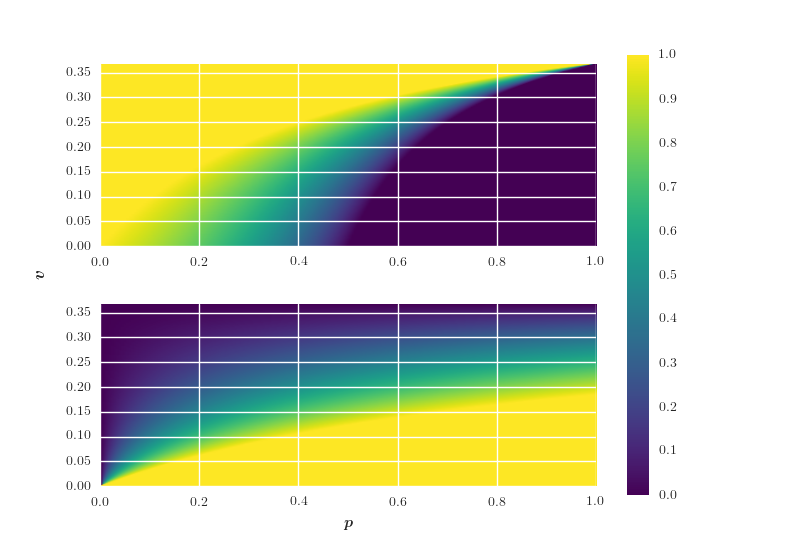
\includegraphics[scale = 0.55]{./figures/b_bounds.png}
\caption{Bounds on $b$ for various values of $p$ and $v$ at $\alpha \rightarrow e$. Top shows lower bounds on $b$ for $RoR_A \geq RoR_B$ and bottom shows upper bounds of $b$ for $RoR_A \geq \frac{b}{2}$.}
\label{fig:b_restrictions}
\end{centering}
\end{figure}

\begin{theorem}
Under proportional budgeting, as $\alpha\rightarrow e$, a necessary and sufficient condition for reward program to be strictly better is a lowerbound on $p$ which increases with $v$.  
And as $p$ increases beyond the lowerbound, the region of allowable $b$ for which the reward program is strictly better becomes larger. 
\end{theorem}
%\proof
%\endproof

Now we generalize the above result for all values of $\alpha$. The conditions are more complex but the results and intuitions are similar. 

\begin{lemma}
Fix $\alpha \in (0, e)$. For any $(p,v)$ pair, there exists some upper bound $b_1 \in [0,1]$ such that for all $b \leq b_1$, $RoR_A \geq \frac{b}{2}$.
\end{lemma}

\proof
We delay the proof of this lemma to first prove a helpful proposition. It is a straightforward computation to see that the condition of $RoR_A \geq \frac{b}{2}$ is equivalent to:
\begin{gather*}
\frac{1}{b}\left(1-\frac{e-\alpha}{b\alpha}\log \left(1+\frac{b\alpha}{e-\alpha} \right) \right) \geq \frac{\alpha(1-(1-p)(1-\alpha v))}{2pe(1-\alpha v)} \\
\iff
g(b; \alpha) \geq h(p, v; \alpha)
\end{gather*}
where we have defined functions $g(b)$ and $h(p,v)$ for fixed $\alpha$ for the above inequalities. 

\begin{proposition}
For a fixed $\alpha$, $g(b)$ is non-increasing for all $b \in (0,1)$. 
\end{proposition}

\proof
We take the derivative of $g$:
\begin{align*}
g'(b) &= \frac{2(e-\alpha)}{b^3 \alpha} \log\left(1+\frac{b\alpha}{e-\alpha} \right) - \frac{1}{b^2}-\frac{1}{b^2\left(1+\frac{b\alpha}{e-\alpha}\right)} \leq 0 \\
&\iff \frac{2(e-\alpha)}{b \alpha} \log\left(1+\frac{b\alpha}{e-\alpha} \right) \leq 1+\frac{1}{1+\frac{b\alpha}{e-\alpha}} \\
&\iff \frac{2\log(1+x)}{x} \leq 1+\frac{1}{1+x}
\end{align*}
where $x = \frac{b\alpha}{e-\alpha}$, and as $b \in (0,1)$, $x \in (0, \frac{\alpha}{e-\alpha})$. We can see that as $x \rightarrow 0$, the above inequality is an equality. 
We represent the LHS of the above equation as $L(x)$ and RHS as $R(x)$. Next we show that $L(x)$ decreases more quickly than $R(x)$ does for positive $x$, thereby proving the proposition.
First show that in the range of $x$ the following holds true:

\beq
\label{eq:eq00}
\left(2-\frac{1}{1+x}\right)^2 \le 2\log(1+x) + 1
\eeq
To show the above observe that at $x\rightarrow 0$ both the LHS and RHS are equal. And it is easy to show that the derivative of LHS is lower than the derivative of RHS for all $x\ge 0$ as shown.
\begin{align*}
& (1+x) + \frac{1}{1+x} \ge 2\\
\implies & 2 - \frac{1}{1+x} \le 1 + x\\
\implies & \left(2-\frac{1}{1+x}\right)\cdot \frac{1}{1+x} \le 1\\
\implies & 2\cdot \left(2-\frac{1}{1+x}\right)\cdot \left(\frac{1}{1+x}\right)^2 \le \frac{2}{1+x}
\end{align*}
The left hand side is the derivative of the above LHS and right hand side is the derivative of the above RHS.

Now we can rearrange Eq.~\ref{eq:eq00} as follows:
\begin{align*}
& \left(2-\frac{1}{1+x}\right)^2 \le 2\log(1+x) + 1\\
\implies & \left(1 + \frac{x}{1+x}\right)^2 \le 2\log(1+x) + 1\\
\implies & \left(\frac{x}{1+x}\right)^2 + \frac{2x}{1+x} \le 2\log(1+x)\\
\implies & 2\left(\frac{x}{1+x} - \log(1+x)\right) \le - \left(\frac{x}{1+x}\right)^2\\
\implies & \frac{2\left(\frac{x}{1+x} - \log(1+x)\right)}{x^2} \le - \left(\frac{1}{1+x}\right)^2
\end{align*}
The left hand side of above is $L'(x)$ and right hand side is $R'(x)$.

\endproof

Thus, $g(b)$ is decreasing in $b$, so for any $(p,v)$ pair, we may compute $h(p, v; \alpha)$, which will then fall into one of the following three cases.
\begin{itemize}
\item
$h(p,v;\alpha) \geq g(0)$. So no value of $b$ makes the reward program profitable.
\item
$h(p,v;\alpha) \leq g(1)$. So any value of $b$ makes the reward program profitable.
\item
$h(p,v;\alpha) = g(b_0)$ for some $b_0 \in (0,1)$. So the reward program is profitable for all $b \leq b_0$ and not otherwise.
\end{itemize}

The above proposition and discussion proves our lemma: for fixed $\alpha$ and any $(p,v)$ pair, there is some upperbound on $b$ s.t. $RoR_A > \frac{b}{2}$. 
\endproof

Now we again look at the conditions for $RoR_A > RoR_B$ to get a lower bound on $b$.  
\begin{lemma}
Fix $\alpha \in (0, e)$. For any $(p,v)$ pair, there exists some lower bound $b_0 \in [0,1]$ such that for all $b \geq b_0$, $RoR_A > RoR_B$.
\end{lemma}

\proof
Let $\frac{b\alpha}{e-\alpha} = x$. Then $RoR_A > RoR_B$ can be evaluated as follows:

\begin{eqnarray}
& p\frac{e}{\alpha}\left(1-\frac{\log(1+x)}{x}\right)(1-\alpha v + 1 - v) - p(1-v) + (1-p)\frac{b}{2}\left(1-\alpha v + 1-v\right) + p(1-v) > 1-v\notag\\
& \implies p\left(1 - \frac{\log(1+x)}{x}\right) + (1-p)\frac{b\alpha}{2e} > \frac{\alpha}{e} \cdot \frac{1-v}{1-\alpha v + 1 - v}\label{eq:ra>rb}
\end{eqnarray}

Since $\alpha$ is a constant, the LHS above is a function of $b$ and $p$. 
Let the LHS above be $L(b,p)$.
We first show that in the range of $b\in [0,1]$, $1 - \frac{\log(1+x)}{x} > \frac{b\alpha}{2e}$ which shows that $L(b,p)$ is increasing in $p$.

\begin{align*}
& 1-\frac{\log(1+x)}{x} > \frac{b\alpha}{2e}\\
\Leftrightarrow & x - \log(1+x) > \frac{b^2\alpha^2}{2e(e-\alpha)}
\end{align*}
Observe that LHS is equal to RHS when $b\rightarrow 0$. 
All we show is that LHS increases faster than RHS in the range of $b\in [0,1]$. 

\begin{align*}
\Leftrightarrow & \left(1 - \frac{1}{1+x}\right) \frac{\alpha}{e-\alpha} > \frac{b\alpha^2}{e(e-\alpha)}\\
\Leftrightarrow & \frac{1}{1+x} > \frac{e-\alpha}{e}\\
\Leftrightarrow & \frac{e}{e-\alpha} > 1 + \frac{b\alpha}{e-\alpha}
\end{align*}
And the last equation is true in the range of $b\in [0,1]$. Hence $L(b,p)$ increases with $p$.

Now we show that $L(b,p)$ increases with $b$ as well. First observe:

\beq
\frac{\partial L(b,p)}{\partial b} = p\left(\frac{\log(1+x) - \frac{x}{1+x}}{x^2}\right)\frac{\alpha}{e-\alpha} + (1-p)\frac{\alpha}{2e}
\notag
\eeq

Thus $\frac{\partial L(b,p)}{\partial b} > 0$ implies:

\begin{align*}
& (1-p)\frac{\alpha}{2e} > p\left(\frac{\frac{x}{1+x} - \log(1+x)}{x^2}\right)\frac{\alpha}{e-\alpha}\\
\Leftrightarrow & (1-p)\frac{b^2\alpha^2}{2e(e-\alpha)} > p \left(1 - \frac{1}{1+x} - \log(1+x)\right)
\end{align*}

Again the LHS and RHS are equal as $b\rightarrow 0$. All we show again is that LHS increases faster as compared to RHS.

\begin{align*}
\Leftrightarrow (1-p)\frac{b\alpha^2}{e(e-\alpha)} > p\left(\frac{1}{(1+x)^2} - \frac{1}{1+x} \right)\frac{\alpha}{e-\alpha}\\
\end{align*}
Clearly RHS is negative when $b\in (0,1]$ and LHS is positive. Hence proved.

Thus $L(b,p)$ is increasing in both $b$ and $p$. And the condition required is $L(b,p)$ is greater than some constant value which depends on $v$.
Hence for any $v$ there exists a smooth $(b_0,p_0)$ curve such that for all $b\ge b_0$ and $p\ge p_0$ revenue rate of reward program merchant is larger.

\endproof

We combine the above two lemmas as before to get the following theorem.

\begin{theorem}
Fix $\alpha \in (0, e)$. 
For any value of $v$, there exists a lowerbound $p_0$ such that for any $p$ greater than $p_0$, there exists a range $(b_0, b_1)$ between $0$ and $1$ such that for all $b$ lying between $b_0$ and $b_1$, offering the reward program is strictly better for $A$. 
\end{theorem}

The above results can be extremely helpful in the following way: if a merchant believes excess loyalty is uniform and has good estimates of its target customer population, \ie, $b$ and $p$ values, it can find the appropriate reward budget ratios $\alpha$, which could make running a reward program strictly better against a traditional pricing competitor. Most importantly, these results show that under mild assumptions on the customer poplation parameters, reward programs can be beneficial in our duopoly model.
